\documentclass[a4paper,12pt]{article}

% Import the deliverable package from common directory
\usepackage{../common/deliverable}

% Tell LaTeX where to find graphics files
\graphicspath{{../common/logos/}{./figures/}{../}}

\usepackage{xspace}
\usepackage{lipsum}

\usepackage{amsmath}
\usepackage{bm}
\usepackage{subcaption}
\usepackage{algorithm}
\usepackage{algorithmic}
\usepackage{multirow}

% Set the deliverable number (without the D prefix, it's added automatically)
\setdeliverableNumber{1.9}

% Begin document
\begin{document}

% Create the title page with the title as argument
\maketitlepage{Report on deal.ii improvements - IV semester}

\newpage

% Main Table using the new environment and command
\begin{deliverableTable}
    \tableEntry{Deliverable title}{Report on deal.ii improvements - IV semester}
    \tableEntry{Deliverable number}{D1.9}
    \tableEntry{Deliverable version}{v1}
    \tableEntry{Date of delivery}{July 31, 2026}
    \tableEntry{Actual date of delivery}{[Actual date]}
    \tableEntry{Nature of deliverable}{Report}
    \tableEntry{Dissemination level}{Public}
    \tableEntry{Work Package}{WP1}
    \tableEntry{Partner responsible}{INPT}
\end{deliverableTable}

% Abstract and Keywords Section
\begin{deliverableTable}
    \tableEntry{Abstract}{\lipsum[1][1-5]}
    \tableEntry{Keywords}{Keyword 1; Keyword 2; Keyword 3; Keyword 4; Keyword 5}
\end{deliverableTable}

\newpage

\begin{documentControl}
    \addVersion{0.1}{July 18, 2026}{Biswajeet Rath}{Initial draft}
    \addVersion{0.2}{[Date]}{[Author name]}{[Description of changes]}
    \addVersion{0.3}{[Date]}{[Author name]}{[Description of changes]}
    \addVersion{1.0}{[Date]}{[Author name]}{Final version}
\end{documentControl}

\subsection*{{Approval Details}}
Approved by: [Name] \\
Approval Date: [Date]

\subsection*{{Distribution List}}
\begin{itemize}
    \item [] - Project Coordinators (PCs)
    \item [] - Work Package Leaders (WPLs)
    \item [] - Steering Committee (SC)
    \item [] - European Commission (EC)
\end{itemize}

\vspace*{2cm}

\disclaimer

\newpage

\tableofcontents % Automatically generated and hyperlinked Table of Contents

\newpage

\section{{Introduction}}

\lipsum[1-2]

\subsection{{Purpose of the Document}}
\lipsum[3]

\subsection{{Structure of the Document}}
\begin{itemize}
    \item Section \ref{sec:section2}: [Section Title]
    \item Section \ref{sec:section3}: [Section Title]
    \item Section \ref{sec:section4}: [Section Title]
    \item Section \ref{sec:section5}: [Section Title]
    \item Section \ref{sec:section6}: [Section Title]
\end{itemize}

\newpage

\section{UNIPI}
\label{sec:section2}
%\lipsum[4-5]
The objective of this work is to develop an implicit hybridizable discontinuous Galerkin (HDG) solver for reduced order one-dimensional blood flow in complex vascular networks within \texttt{deal.II} library. The implementation combines the Harten Lax van Leer (HLL) numerical flux integrated with the SUNDIALS IDA solver for efficient implicit time integration. We implement a fully coupled monolithic Newton solver, eliminating the need for sub-Newton iterations within each global Newton step.

\subsection{Governing System}
%\lipsum[6]
We consider the one-dimensional blood flow equations parameterized along a centerline tangent vector $\bm b(\bm x)$. The compact vector form of the conservation system is given by:
\begin{equation}
  \partial_t \mathbf{w} + \nabla \cdot \left(\bm b(\bm{x})  \mathbf{F}(\mathbf{w})\right) = \mathbf{S}(\mathbf{w}), \qquad
  \mathbf{w} = \begin{pmatrix} A \\ U \end{pmatrix}, \qquad
  \mathbf{S}(\mathbf{w}) = \begin{pmatrix} 0 \\ - \frac{f U}{A} \end{pmatrix},
\end{equation}
where $A(x,t)$ is the cross-sectional area, $U(x,t)$ is the mean velocity, $\rho$ is the blood density, and
$f = 2(\zeta+2)\,\mu\,\pi$ is the viscous friction coefficient
with dynamic viscosity $\mu$ and velocity-profile parameter
$\zeta$. 
The non-linear physical flux vector $\mathbf{F}(\mathbf{w})$ is:
\begin{equation}
  \mathbf{F}(\mathbf{w}) = \begin{pmatrix} F_A(\mathbf{w}) \\ F_U(\mathbf{w}) \end{pmatrix} = \begin{pmatrix} A U \\ \frac{U^2}{2} + \frac{1}{\rho} P(A) \end{pmatrix}.
\end{equation}
The arterial wall mechanics are governed by the tube law
\begin{align*}
P(A,x) - P_0 = P_d + \frac{\beta}{A_d(x)}
\left[ (A^m - A_d(x)^m) \right], \text{ with }  \beta = 4/3 \sqrt{\pi} E h_w(x),
\end{align*}
where $P_0 $ is the external pressure, $P_d$ is the diastolic pressure,
$E$ is the wall Young's modulus,
$h_w(x)$ is the wall thickness, and
$A_d(x)$ is the \emph{local diastolic area}, tube law constant $m =0.5$.

\subsubsection{HDG Implementation}
The main components implemented in the HDG solver are summarized below:
\begin{itemize}
    \item Implemented the Hybridizable Discontinuous Galerkin (HDG) discretization for the one-dimensional blood flow equations.
    \item Implemented the Harten--Lax--van Leer (HLL) numerical flux for communication between neighboring elements.
    \item Developed a unified trace formulation for
    \begin{itemize}
        \item interior interfaces,
        \item inflow and outlet boundary conditions, and
        \item vascular junctions (including bifurcations).
    \end{itemize}
    
    \item Incorporated physiological outlet models, including single-resistance and three-element Windkessel (RCR) boundary conditions.  
    \item Coupled the semi-discrete HDG system with the \textsc{SUNDIALS} IDA solver for fully implicit time integration.
    \item Assembled the complete residual and analytical Jacobian required by Newton's method for efficient nonlinear solution.
\end{itemize}


\subsection{Results}
%\lipsum[7]
The developed HDG solver has been validated using the well-established 37-artery human systemic network benchmark proposed by Alastruey et al.~\cite{matthys2007pulse}. The network consists of 37 arterial segments connected through 21 bifurcations and is driven by a physiological inflow waveform. At each terminal vessel, a single-resistance outlet condition,
\[
P-P_{\mathrm{out}} = RQ,
\]
is imposed, while the bifurcations are coupled through the proposed HDG trace formulation by enforcing mass conservation and continuity of total pressure.

\begin{figure}[ht]
    \centering
    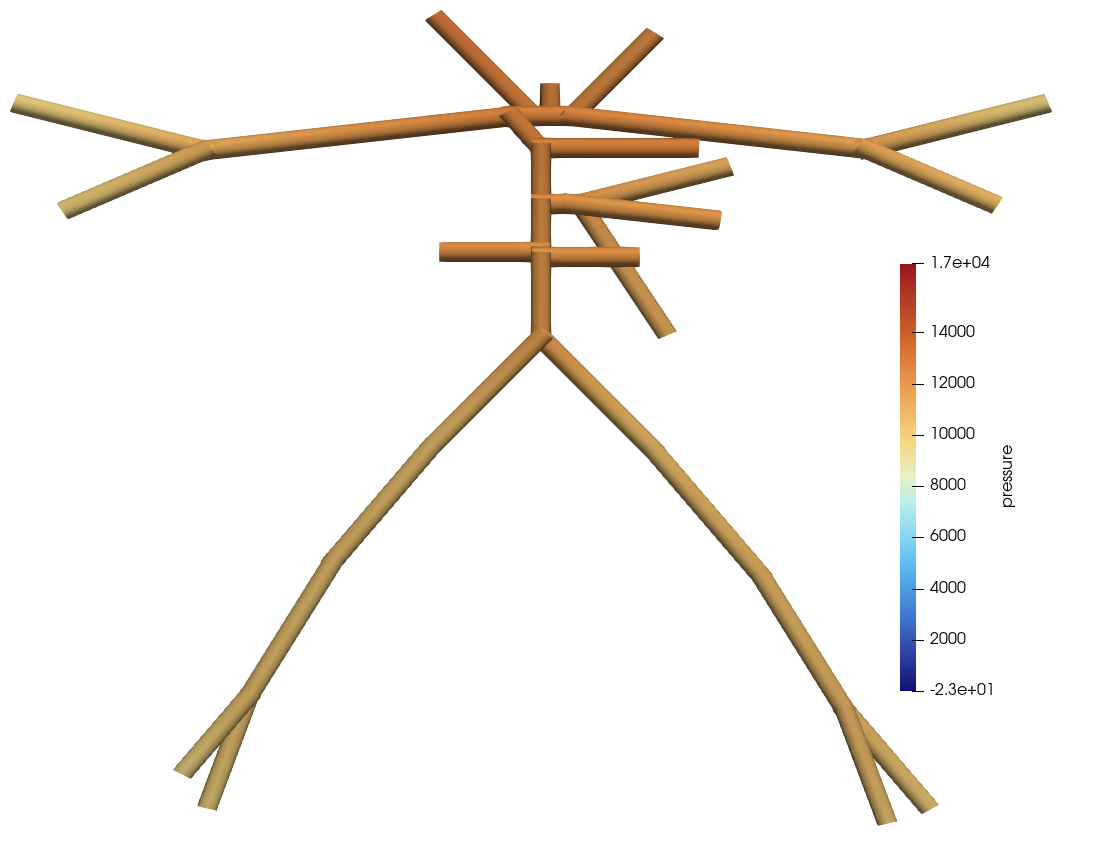
\includegraphics[width=0.45\linewidth]{figures/pressure_at_t14.155_37_arteries.png}
    \caption{Pressure distribution in the 37-artery benchmark at $t\approx14.155\,\mathrm{s}$.}
    \label{fig:37network}
\end{figure}

The numerical solution is validated against the finite-volume benchmark of Boileau \emph{et al.}~\cite{boileau2015benchmark}. For comparison, the pressure, flow rate, and cross-sectional area are monitored at the midpoint of the thoracic aorta II, which is one of the major arteries close to the heart. Figure~\ref{fig:thoracic_results} shows an excellent agreement of the computed solution with the benchmark reference throughout one cardiac cycle.

\begin{figure}[ht]
    \centering
    \begin{subfigure}[b]{0.32\textwidth}
        \centering
        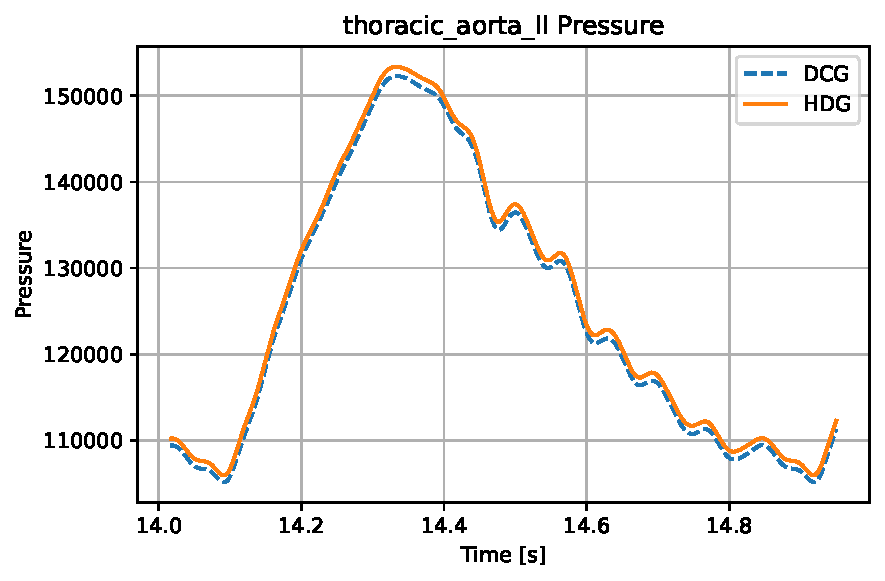
\includegraphics[width=\linewidth]{figures/thoracic_aorta_II_pressure.pdf}
        \caption{Pressure}
    \end{subfigure}
    \hfill
    \begin{subfigure}[b]{0.32\textwidth}
        \centering
        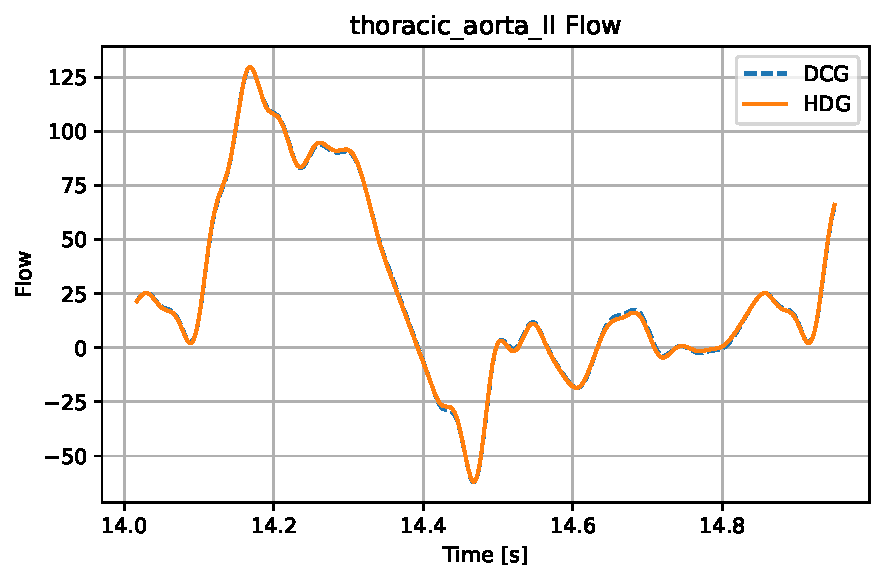
\includegraphics[width=\linewidth]{figures/thoracic_aorta_II_flow.pdf}
        \caption{Flow rate}
    \end{subfigure}
    \hfill
    \begin{subfigure}[b]{0.32\textwidth}
        \centering
        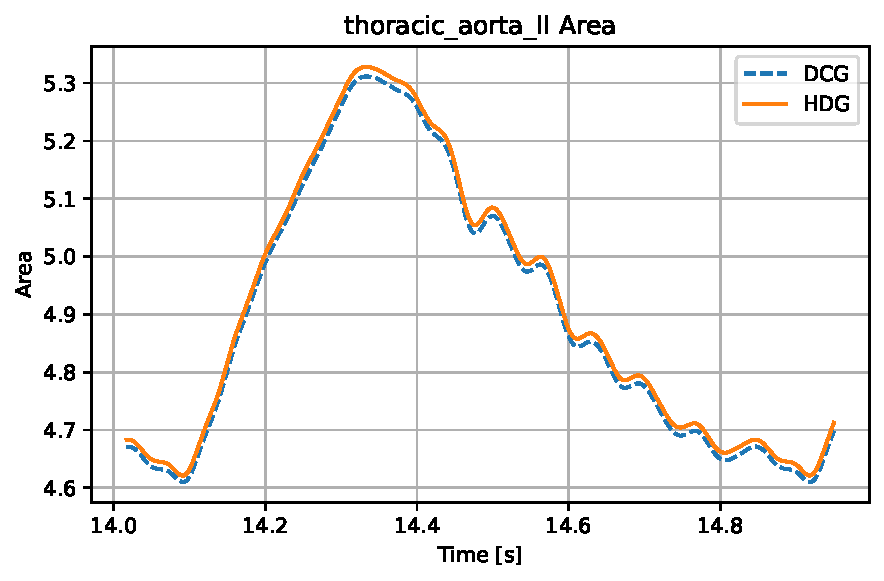
\includegraphics[width=\linewidth]{figures/thoracic_aorta_II_area.pdf}
        \caption{Area}
    \end{subfigure}
    \caption{Comparison of pressure, flow rate, and cross-sectional area at the midpoint of the thoracic aorta II over one cardiac cycle.}
    \label{fig:thoracic_results}
\end{figure}

To further demonstrate that the numerical solution is independent of the spatial discretization, a mesh independence study was carried out using successive mesh refinements. As shown in Figure~\ref{fig:mesh_independence}, the numerical solution converges rapidly, with negligible differences observed for the finer meshes. This confirms that the reported results are not artifacts of the computational mesh.

\begin{figure}[ht]
    \centering
    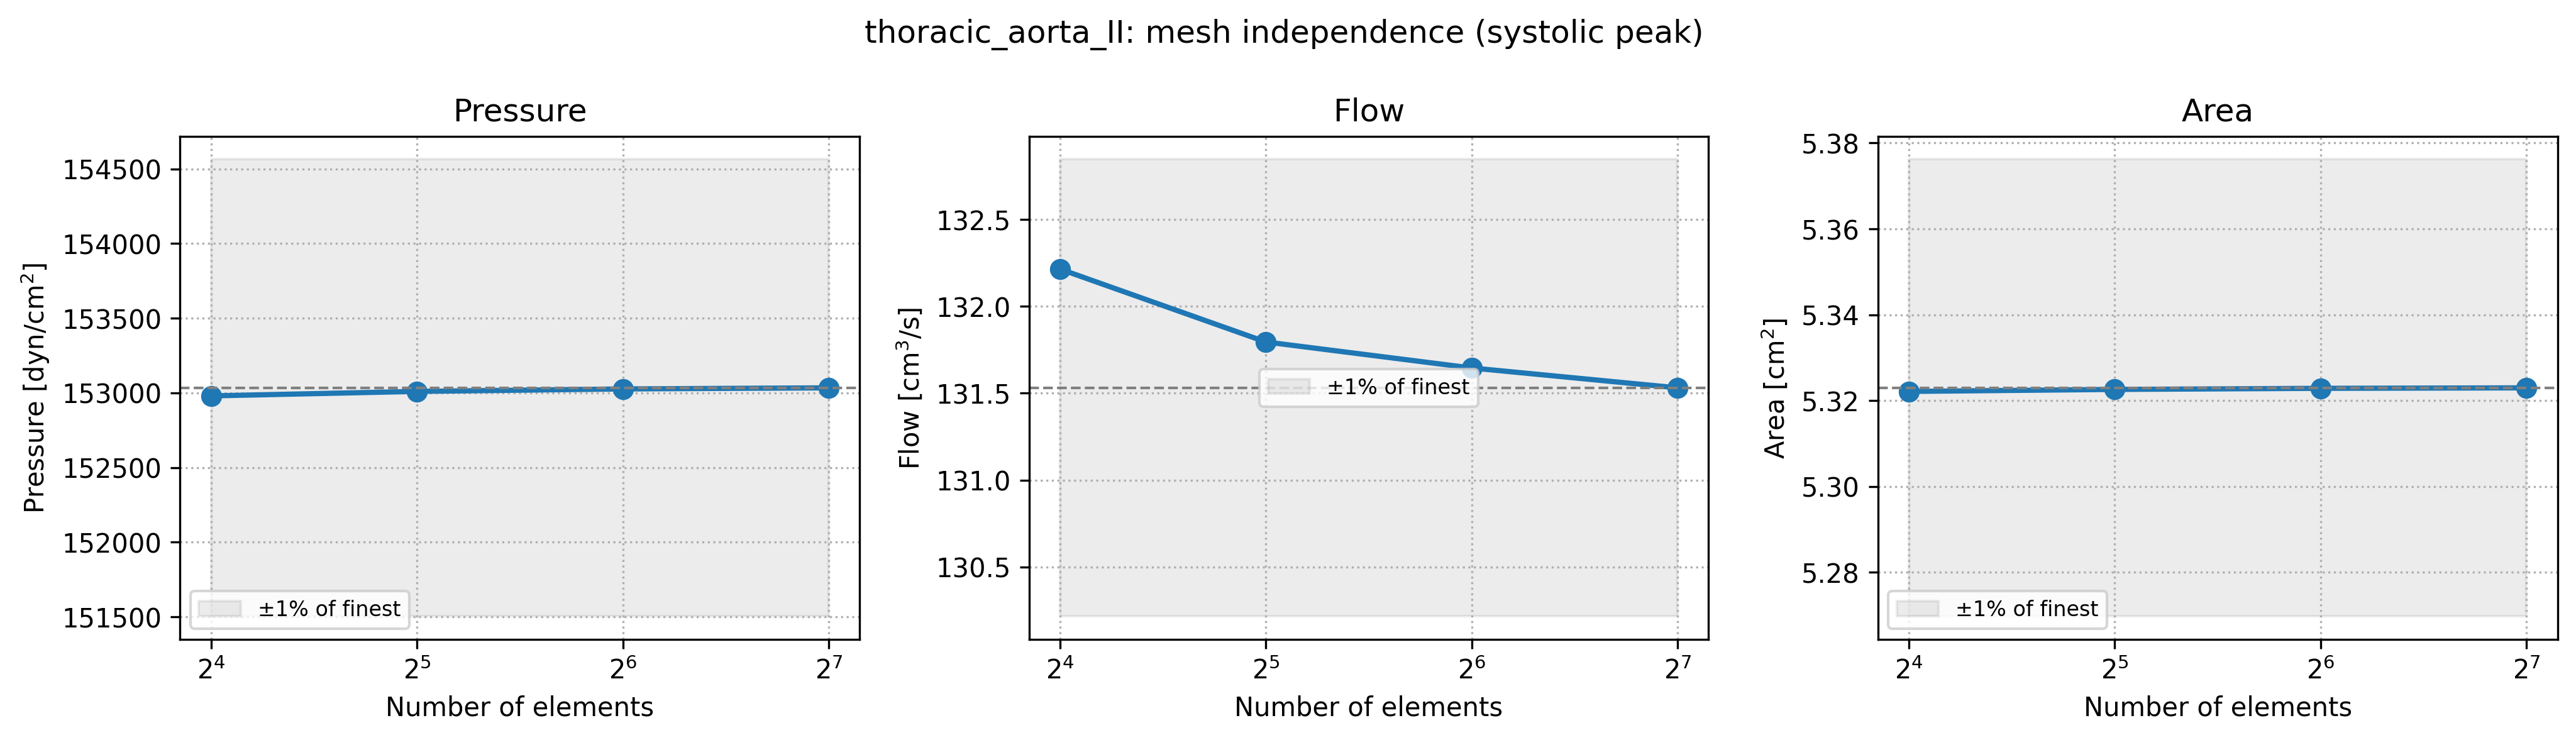
\includegraphics[width=\linewidth]{figures/results_37_thoracic_aorta_II_mesh_independence.png}
    \caption{Mesh independence study for the thoracic aorta II.}
    \label{fig:mesh_independence}
\end{figure}


\newpage


\section{INPT}
\label{sec:section3}

%\lipsum[8-9]
In this section, we highlight some of the recent work carried out with the MUMPS direct solver in the context of the dealii-X project. The primary objective has been to evaluate the use of low rank approximation techniques and mixed precision algorithms for organ simulation problems arising from \texttt{deal.II}. The following sections provide a brief background on the theoretical aspect and the recent features available in MUMPS with performance results on a sample matrix. The sample matrix is a medium resolution matrix for the brain indentation problem obtained from our collaborators at FAU Erlangen. The problem consists of 3 million degrees of freedom and $6.2\times 10^8$ elements. We solve the problem with the direct solver for a desired accuracy of $10^{-10}$. All the results in this section have been obtained on 1 compute node with 24MPIx8th configuration on the CPU partition of the Kairos cluster in Toulouse [].

\subsection{Low Rank Approximation}
% \begin{itemize}[left=1em, itemsep=0pt, topsep=0pt] 
%     \item \lipsum[10][1-2]
%     \item \lipsum[10][3-4]
%     \item \lipsum[10][5-6]
% \end{itemize}
Data sparsity within a matrix results in a low numerical rank. We can take advantage of this fact by using a low-rank approximation for the respective matrix. MUMPS uses the block row rank (BLR) approach to represent low rank blocks within the dense frontal matrices during the numerical factorization phase []. This can result in a significant reduction in memory consumption and consequently lower operation count. The accuracy of the low rank representation is controlled by a user-defined parameter $\varepsilon$, known as the BLR threshold, 
\begin{equation}\label{BLR_error}
    \left\lVert A-X\Sigma Y^T\right\rVert_2 \leq \varepsilon,
\end{equation}
where $X\Sigma Y^T$ represents the truncated SVD of $A$.
Additionally, MUMPS is capable of storing different columns of the factorized block, i.e. $X$ and $Y$ in the above example, at different precisions, based on the magnitude of the corresponding singular value. This is referred to as adaptive precision BLR [] and leads to a further reduction in memory footprint.

\begin{figure}
    \begin{subfigure}[h]{0.48\textwidth}
        \centering
        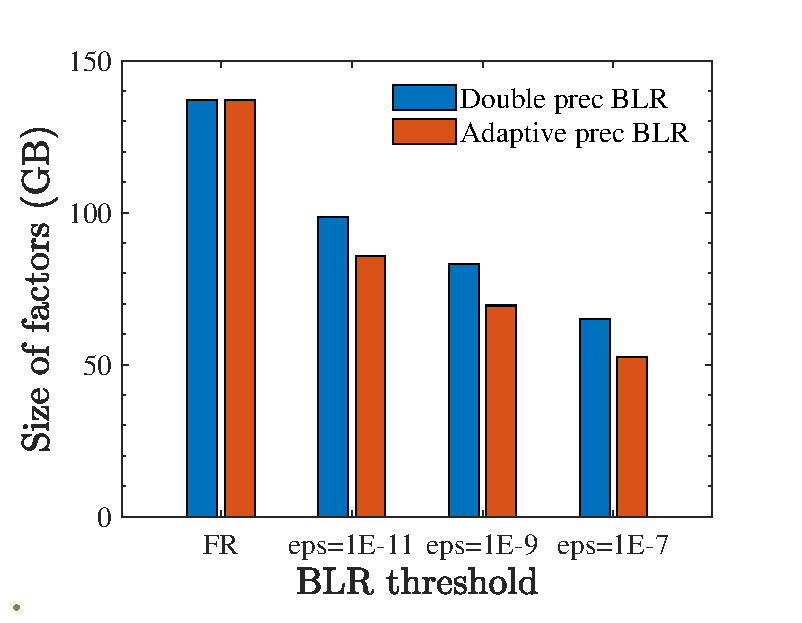
\includegraphics[width=1\textwidth]{brain_LU_size}
        \caption{}
        \label{LU_size}
    \end{subfigure}
    \hfill
    \begin{subfigure}[h]{0.48\textwidth}
        \centering
        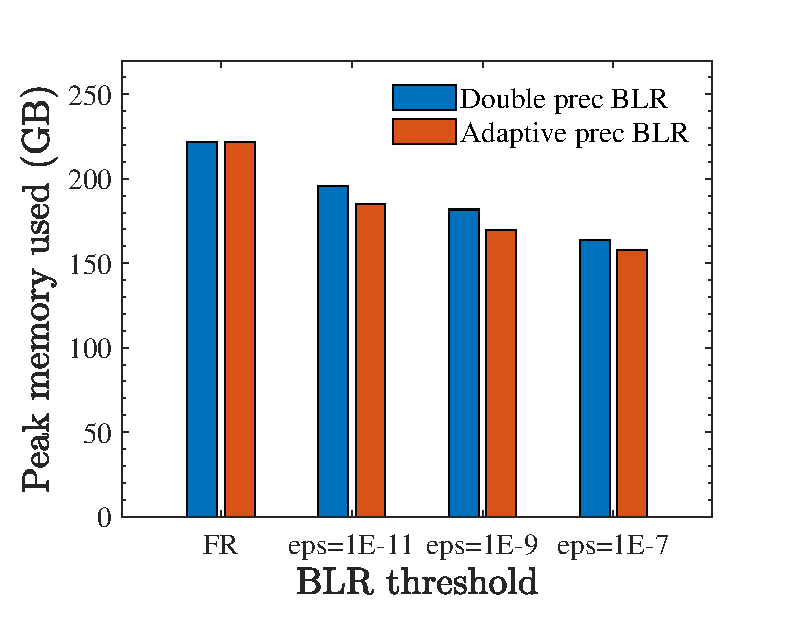
\includegraphics[width=1\textwidth]{brain_peak_mem}
        \caption{}
        \label{peak_mem}
    \end{subfigure}
    \centering
    \caption{Memory study: (a) size of $LU$ factors and (b) peak memory usage during factorization. The bar graphs show the comparison between double precision and adaptive precision BLR for different values of the BLR threshold $\varepsilon$. FR refers to the full rank case.}
    \label{fig:brain_mem}
\end{figure}

\begin{figure}
    \begin{subfigure}[h]{0.48\textwidth}
        \centering
        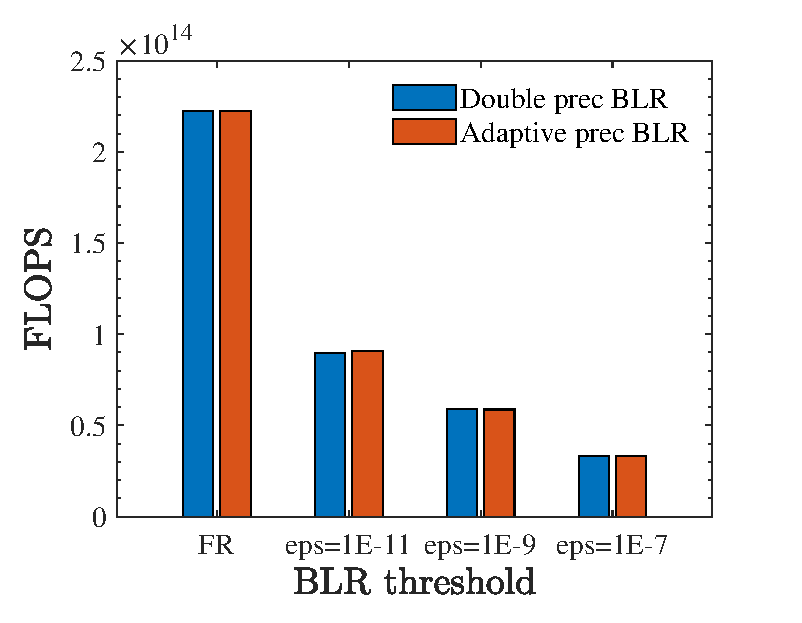
\includegraphics[width=1\textwidth]{figures/brain_flops}
        \caption{}
        \label{flops}
    \end{subfigure}
    \hfill
    \begin{subfigure}[h]{0.48\textwidth}
        \centering
        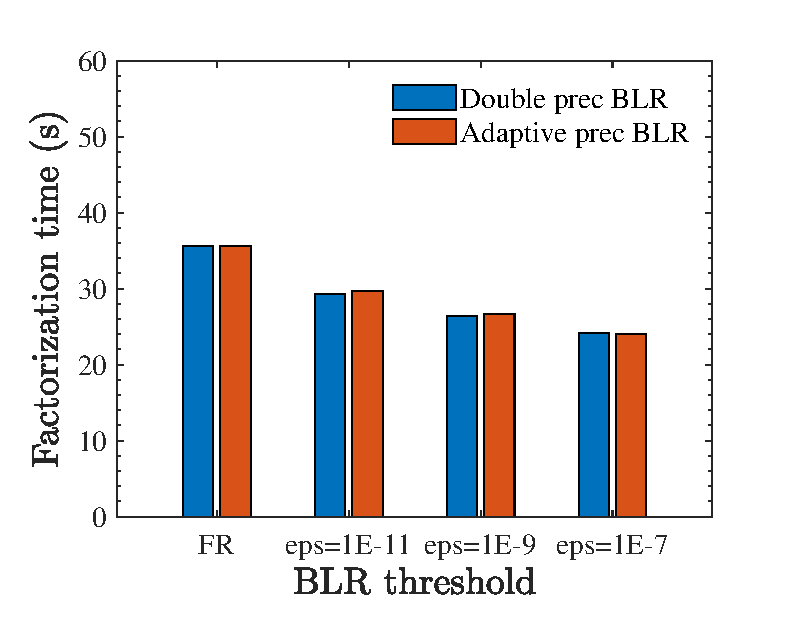
\includegraphics[width=1\textwidth]{figures/brain_t_fac}
        \caption{}
        \label{t_fac}
    \end{subfigure}
    \centering
    \caption{(a) Operation count and (b) elapsed time during the numerical factorization phase. The bar graphs show the comparison between double precision and adaptive precision BLR for different values of the BLR threshold $\varepsilon$. FR refers to the full rank case.}
    \label{fig:brain_fac}
\end{figure}

Figure \ref{fig:brain_mem} illustrates the memory footprint for the sparse direct solver for different values of the BLR threshold $\varepsilon$. We can observe that with the introduction of BLR, the size of the $LU$ factors reduces by $28\%$. The gain goes up to $50\%$ for the largest possible $\varepsilon$ of $10^{-7}$. Using adaptive precision BLR further brings down the memory consumption by around $13\%$. Similarly, the peak memory used during the factorization process reduces by $26\%$ for the largest BLR threshold compared to the full rank case.

Figure \ref{fig:brain_fac} highlights the operation counts and factorization time for solving the brain matrix problem. The number of FLOPS reduces drastically by $60\%$ owing to BLR compression. It goes down consistently and achieves a gain of $85\%$ for the largest $\varepsilon$ value. The time elapsed during factorization reduces by $32\%$ for $\varepsilon=10^{-7}$ compared to the full rank case. These results clearly illustrate the benefits of using low rank approximation techniques both in terms of reducing complexity and improving performance. This makes the use of MUMPS possible even for memory intensive applications.

\subsection{Mixed Precision Iterative Refinement}
%\lipsum[11]
Mixed precision algorithms refer to the use of multiple floating point formats with different precisions within a given algorithm. In this work, we will focus on mixed LU-IR where we perform certain steps of the iterative refinement algorithm at a lower precision. The goal of iterative refinement is to recover the loss in accuracy due to approximate computing. Algorithm \ref{algorithm_1} lays out the procedure for performing mixed LU-IR with two precisions: single (fp32) and double (fp64). The idea is to perform the time and memory intensive steps at a lower precision in order to reduce the overall memory footprint and the execution time of the algorithm. 
\begin{algorithm}
	\caption{Mixed LU-IR}
	\label{algorithm_1}
	\begin{algorithmic}[1]
	\STATE Factorize $A=LU$ \hfill in precision fp32\\
    \STATE Solve $Ax_1=b$ via $x_1=U^{-1}(L^{-1}b)$ \hfill in precision fp32\\
    \STATE repeat \\
        \STATE \quad $r_i = b - Ax_i$ \hfill in precision fp64\\
        \STATE \quad Solve $Ad_i=r_i$ via $d_i=U^{-1}(L^{-1}r_i)$ \hfill in precision fp32\\
        \STATE \quad $x_{i+1} = x_i + d_i$ \hfill in precision fp64\\
    \STATE until convergence \\
	\end{algorithmic}
\end{algorithm}

The above algorithm results in $\mathcal{O}(n^3)$ operations in single precision and $\mathcal{O}(n^2)$ operations in double precision per iteration. It is guaranteed to converge in double precision given that $\kappa(A) < \frac{1}{u_{\text{fp32}}}=1.6 \times 10^7$, where $\kappa(A)$ is the condition number of the matrix $A$ and $u_{\text{fp32}}$ is the unit round-off for single precision float [].

\begin{table}[htbp]
\centering  
\caption{Performance comparison between double precision and single precision factorization with iterative refinement.}  
\begin{center}
\begin{tabular}{ p{1.5cm}| p{1.5cm}| p{1cm}| p{1.7cm}| p{1cm}| p{1cm}| p{1cm}| p{1.2cm}| p{1.2cm} }
%\begin{tabular}{ c|c|c|c|c|c|c|c|c }
 % \hline
 \hline
 \hline
 \multirow{2}{2em}{} & \multicolumn{2}{c|}{Memory study (GB)} & \multirow{2}{2em}{FLOPS} & \multicolumn{3}{c|}{Elapsed time (sec)} & \multicolumn{2}{c}{Bwd error}\\ 
 & Size $\vert LU\vert$ & Memory used & & Facto & Solve & LU-IR (nb) & Initial & LU-IR\\
 \hline
 \hline
 Full rank (FR) & 137.04 & 221.91 & 2.23E+14 & 35.55 & 0.21 & $-$ & 2.81E-16 & $-$\\
 \hline
 BLR $\varepsilon$=1E-7 & 64.88 & 163.68 & 3.33E+13 & 24.17 & 0.12 & 8.19 (3) & 3.35E-6 & 1.94E-13\\
 \hline
 \multicolumn{9}{c}{Single precision factorization} \\
 \hline
 Full rank (FR) & 68.52 & 112.36 & 2.23E+14 & 18.43 & 0.12 & 8.08 (3) & 5.11E-11 & 1.39E-12\\
 \hline
 BLR $\varepsilon$=1E-7 & 32.44 & 84.06 & 3.33E+13 & 13.08 & 0.08 & 9.37 (4) & 2.84E-6 & 1.91E-14\\
 \hline
 \hline
\end{tabular}  
\end{center}
\label{table:SinD-IR}
\end{table}

Table \ref{table:SinD-IR} captures the different quantities of interest and compares them for double precision and single precision factorization with iterative refinement. 
%Single in double refers to performing single precision factorization within a double precision instance of MUMPS (algorithm \ref{algorithm_1}). 
We are able to recover the loss in accuracy by employing the iterative refinement technique. We can observe that by utilizing the mixed LU-IR approach of algorithm \ref{algorithm_1}, we are able to reduce the memory consumption and factorization time by nearly half. Thus, by combining mixed LU-IR with BLR compression, we can bring down memory consumption by $77\%$ and factorization time by $63\%$. This will allow us to use fewer computational resources even for larger problems.

We plan to further investigate the use of GPU acceleration features of MUMPS to factorize the dense frontal matrices. We are also working on the postprocess BLR feature, which allows us to compress the low rank blocks on the CPU after the full rank factorization has been carried out on the GPU. Finally, we plan to extend the study to more organ simulations such as problems involving the liver or the lungs. 

\newpage

\section{SISSA}
\label{sec:section4}

% \lipsum[12-13]

% \begin{center}
%     \begin{table}[h!]
%     \small
%     \caption{[Table Caption]}
%     \renewcommand{\arraystretch}{1.25}
%     \label{tab:example_table}
%     \begin{tabular}{|l|l|l|c|}
%     \hline
%     \textbf{Column 1} & \textbf{Column 2} & \textbf{Column 3} & \textbf{Column 4} \\
%     \hline
%     Item 1 & Description & Category & Value \\
%     Item 2 & Description & Category & Value \\
%     Item 3 & Description & Category & Value \\
%     \hline
%     \end{tabular}
%     \end{table}
% \end{center}

\subsection{Polygonal Discretization Module}
The polygonal discretization activity defined in Work Package 1.3 aims to integrate general-mesh discretization capabilities into \texttt{deal.II}, with particular emphasis on discontinuous Galerkin methods on agglomerated polygonal and polyhedral meshes and on the automatic construction of coarse polygonal grid hierarchies. Deliverable D1.5 introduced the external \texttt{Polydeal} library and described a Poisson tutorial on agglomerated polytopic meshes. Deliverable D1.7 subsequently reported the testing and validation of the library, the opening of a separate, self-contained Code Gallery contribution through pull request \#233, and the ongoing refactoring of reusable components in preparation for their integration into \texttt{deal.II}. During the present reporting period, the Code Gallery contribution was reviewed and merged, and the complete \texttt{agglomeration\_poisson} program, its documentation, and its numerical results became publicly available on the official \texttt{deal.II} Code Gallery page. A follow-up documentation update improving figure rendering and page layout was subsequently submitted through pull request \#244.

In parallel, the integration activity announced in D1.7 has progressed to a concrete submission to the \texttt{deal.II} core library. The central reusable components originating from \texttt{Polydeal} were separated from application-specific code, adapted to \texttt{deal.II} interfaces and coding conventions, and extended into a framework for DG discretizations on agglomerated meshes. The resulting \texttt{deal.II} pull request \#19891 includes agglomeration management, \texttt{deal.II}-style accessor and iterator interfaces, agglomerated degree-of-freedom and sparsity-pattern construction, agglomeration-aware mapping and quadrature, and R-tree-based hierarchical agglomeration. At the reporting date, the pull request is open and under review. A detailed description of this integration activity is provided in Deliverable D1.8, Polygonal discretization in deal.II – II.

\subsection{Unfitted space–time DG method on moving domains}
Building on the agglomeration-based polygonal discretization framework developed in Work Package 1.3, related theoretical work has extended the same general-mesh DG philosophy to parabolic problems posed on moving domains. The evolving physical domain is embedded in a fixed background space–time mesh and described by a time-dependent level-set function, thereby avoiding the need to remesh the computational domain at every time step. In this setting, agglomeration plays a closely related but different role from its use in the construction of coarse polygonal grid hierarchies: background cells whose intersection with the physical domain is arbitrarily small are merged with suitable neighbouring elements to form robust polytopic space–time elements. Under the geometric assumptions used in the analysis, the resulting polytopic space–time elements satisfy bounds that are uniform with respect to the cut configuration. This work therefore extends the agglomeration concepts developed in Work Package 1.3 to unfitted, time-dependent geometries. A preliminary numerical implementation has also been developed to illustrate the resulting mesh construction and discrete solution (Fig. \ref{fig:sissa_mesh}).

\begin{figure}
    \begin{subfigure}[h]{0.48\textwidth}
        \centering
        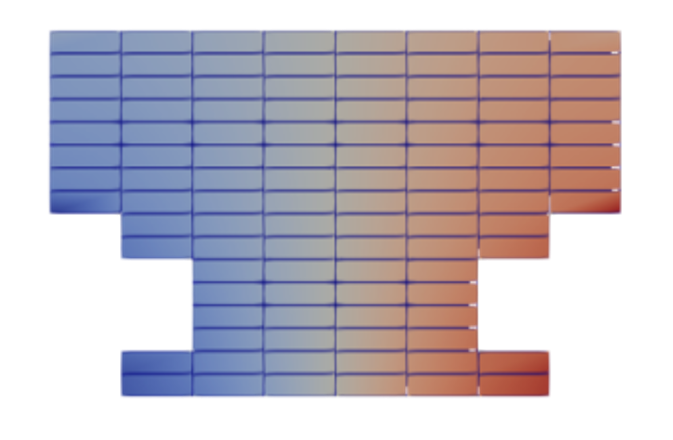
\includegraphics[width=1\textwidth]{figures/bg_mesh.png}
        \caption{}
        \label{flops}
    \end{subfigure}
    \hfill
    \begin{subfigure}[h]{0.48\textwidth}
        \centering
        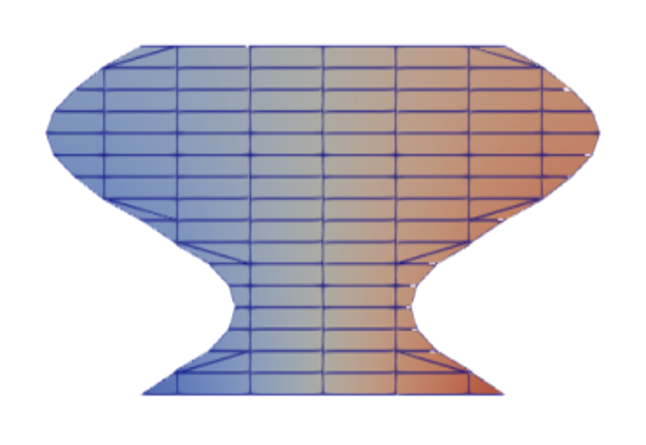
\includegraphics[width=1\textwidth]{figures/cut_mesh.png}
        \caption{}
        \label{t_fac}
    \end{subfigure}
    \centering
    \caption{Illustration of the unfitted space–time discretization. Left: the background space–time mesh before restriction to the physical domain. Right: the active cut mesh and a representative numerical solution on the time-dependent physical domain.}
    \label{fig:sissa_mesh}
\end{figure}

A space–time DG formulation has been developed on the resulting agglomerated mesh. Stability has been established through coercivity and inf-sup estimates that are uniform with respect to the position of the moving boundary relative to the background mesh. An a priori error estimate has also been derived in a DG energy norm whose spatial component controls the broken $H^1$-seminorm. For fixed polynomial degrees, the estimate is optimal with respect to both the spatial mesh size and the time-step size. The corresponding $L^2$-error analysis has not yet been completed and constitutes the next theoretical step.



\newpage

\section{RUB}
\label{sec:section5}

\lipsum[14-15]

\subsection{{[Subsection Title]}}
\lipsum[16]

\subsection{{[Subsection Title]}}
\begin{itemize}[left=1em, itemsep=0pt, topsep=0pt] 
    \item \textbf{[Item Title]}: \lipsum[17][1-2]
    \item \textbf{[Item Title]}: \lipsum[17][3-4]
    \item \textbf{[Item Title]}: \lipsum[17][5-6]
\end{itemize}

\newpage

\section{UNITOV}
\label{sec:section6}

\lipsum[18-19]

\begin{center}
\resizebox{\textwidth}{!}{
\begin{tabular}{|l|l|l|}
\hline
\textbf{Column 1} & \textbf{Column 2} & \textbf{Column 3} \\
\hline
Item 1 & Description & Value \\
\hline
Item 2 & Description & Value \\
\hline
Item 3 & Description & Value \\
\hline
\end{tabular}}
\label{tab:example_table2}
\end{center}

\newpage 

\section{{Conclusion}} \label{sec:conclusion}

\lipsum[20]

\label{MyLastPage}

\end{document}
